\section{Sistema Proposto}

O sistema proposto foi desenvolvido para comparar o desempenho de uma instância única do PostgreSQL 
com um ambiente em cluster utilizando o Citus.

O benchmark utilizado será o TPC-C, desenvolvidos pelo TPC (Transaction Processing Council),
amplamente reconhecido como um padrão do mercado para avaliar desempenho e escalabilidade de sistemas 
de banco de dados. A execução do benchmark será intermediada pelo framework HammerDB.
Utilizaremos o grafana e o prometheus para monitorar o sistema durante os testes.

Para garantir fácil reprodutibilidade e configuração, 
ambos os ambientes serão configurados utilizando o \textbf{Docker Compose}.

\subsection{Ferramentas Utilizadas}
\begin{itemize}
    \item \textbf{Docker Compose:} 
	Ferramenta de orquestração de containers empregada para configurar e iniciar facilmente os ambientes de banco de dados, 
	tanto para a instância única quanto para o cluster.
	
	\item \textbf{PostgreSQL:} 
	Utilizado como sistema gerenciador de banco de dados relacional base,
	tanto no modo standalone quanto no cluster.
    
    \item \textbf{Citus:} 
	Extensão do PostgreSQL que permite a distribuição dos dados e consultas entre múltiplos nós,
	viabilizando o escalonamento horizontal do banco de dados.
    
    \item \textbf{Grafana e Prometheus:} 
	Utilizados para monitoramento e análise de métricas do sistema. 
	O Prometheus coleta e armazena as métricas do PostgreSQL, enquanto o Grafana fornece dashboards interativos,
	para visualização em tempo real do comportamento do sistema.
    
    \item \textbf{HammerDB:}
	Framework de benchmarking utilizado para executar testes de carga nos bancos de dados.
	Foi empregado o benchmark TPC-C, 
	reconhecido como padrão do mercado para avaliação de desempenho e escalabilidade de sistemas de banco de dados.

	\item \textbf{TPC-C:}
	O TPC-C é um benchmark amplamente utilizado para medir o desempenho de sistemas de banco de dados em ambientes 
	de processamento de transações online (OLTP). Ele simula o funcionamento de uma empresa atacadista,
	incluindo operações como criação de pedidos, pagamentos, entregas e controle de estoque,
	por meio de cinco tipos de transações típicas do dia a dia empresarial.
	O teste avalia a capacidade do sistema de processar grandes volumes de transações simultâneas,
	refletindo cenários reais de negócios, e utiliza como principal métrica o número de transações por minuto (tpmC),
	permitindo comparar a performance e escalabilidade de diferentes soluções de banco de dados.
	
	O esquema relacional do TPC-C é o seguinte:
	\begin{figure}[H]
		\centering
		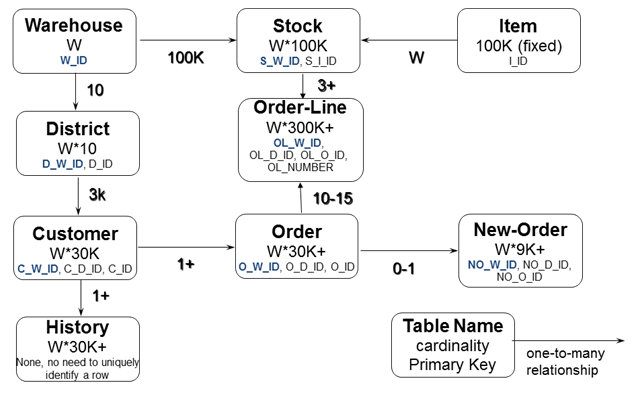
\includegraphics[width=0.8\textwidth]{imgs/ch3-2.png}
		\caption{obtido em: https://www.hammerdb.com/docs3.3/ch03s05.html}
		\label{fig:tpc-c}
	\end{figure}
\end{itemize}

\section{Implementação}

O sistema foi implementado utilizando o Docker Compose, com as ferramentas explicadas na sessão anterior,
e está disponível no repositório do projeto.

Os scripts de inicialização dos ambientes e execução dos benchmarks foram automatizados,
facilitando a replicação dos experimentos e a coleta dos resultados.

Os comandos para reproduzir o sistema e executar o benchmark estão disponíveis no readme do repositório.